% !TeX root = ../../../main.tex
\ChFiveHeadingOnly
\subsubsection{Cohort Demographics}
\label{ch05:sec:cohort-demographics}

For demographic extraction, we used an LLM-based query to retrieve age, sex, and ethnicity for each case.
The prompt instructed the model to report age in years; sex as \texttt{Male}, \texttt{Female}, a free-text category, or \texttt{Not Specified}; and ethnicity according to U.S.\ Census categories or \texttt{Not Specified} (full prompt in Supplementary Material, Section~\ref{ch05:apd:demographics-prompt}).
\ChFiveRebuttal{
The demographic fields are LLM-extracted or LLM-mapped descriptors from the case-report narrative. They should not be interpreted as independently verified biological sex at birth, self-identified race or ethnicity, or population-representative demographic measurements.
}

Across PMOA-TTS, the median age is 47 years, with peaks at 5-year intervals, consistent with rounded age reporting in clinical text (Figure~\ref{ch05:fig:demo}).
The distribution of LLM-extracted sex descriptors is approximately balanced (52\% male, 47\% female, 1\% Not Specified).
\ChFiveRebuttal{
Ethnicity was not specified in 89\% of reports. Among reports with an extracted ethnicity category, White/Caucasian and Asian were the most frequent. Given the extensive missingness and the non-population-based nature of case reports, these proportions should not be interpreted as population prevalence or attributed to a specific underlying cause.
}


% !TeX root = ../../../main.tex
\begin{figure}[htbp]
\begin{ChFiveFloatBody}

  \centering
  \begin{minipage}[t]{0.49\linewidth}
    \centering
    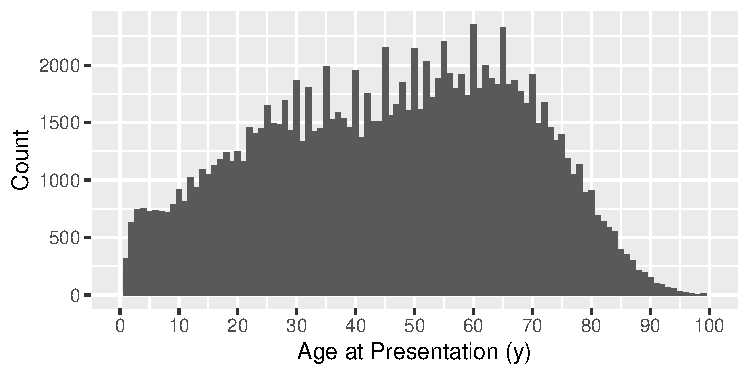
\includegraphics[width=\linewidth]{Chapters/chapter-05/images/Scientific_data/Plots_tables/125k_age.pdf}
  \end{minipage}\hfill
  \begin{minipage}[t]{0.49\linewidth}
    \centering
    \scriptsize
    \begin{tabular}{l r}
      \toprule
      \textbf{Characteristic} & \textbf{Percent (\%)}\\
      \midrule
      \multicolumn{2}{l}{\textbf{Sex}}\\
      \quad Male & 52\\
      \quad Female & 47\\
      \quad Not Specified & 1\\
      \midrule
      \multicolumn{2}{l}{\textbf{Ethnicity}}\\
      \quad White/Caucasian & 5\\
      \quad Asian & 3\\
      \quad African & 1\\
      \quad Other & 2\\
      \quad Not Specified & 89\\
      \bottomrule
    \end{tabular}
  \end{minipage}
  
  
  

\end{ChFiveFloatBody}
\caption{\ChFiveRebuttal{Age distribution and LLM-mapped/extracted demographic descriptors for 124{,}349 PMOA-TTS case reports.}}\ChFiveFloatLabel{ch05:fig:demo}
\end{figure}



